\chapter{Funkcja celu -- porównanie barwy dźwięku} \label{target_function_chapter}

Aby stopniowo dostosować graf przetwarzania sygnałów zaimplementowany 
w rozdziale~\ref{dsp_graph_chapter} do imitowania zadanej próbki dźwięku,
należy wykorzystać funkcję celu, która maleje wraz ze wzrostem podobieństwa
barwy dźwięku między próbki zadaną i sygnałem generowanym przez graf. 

\begin{figure}[H]
    \centering
    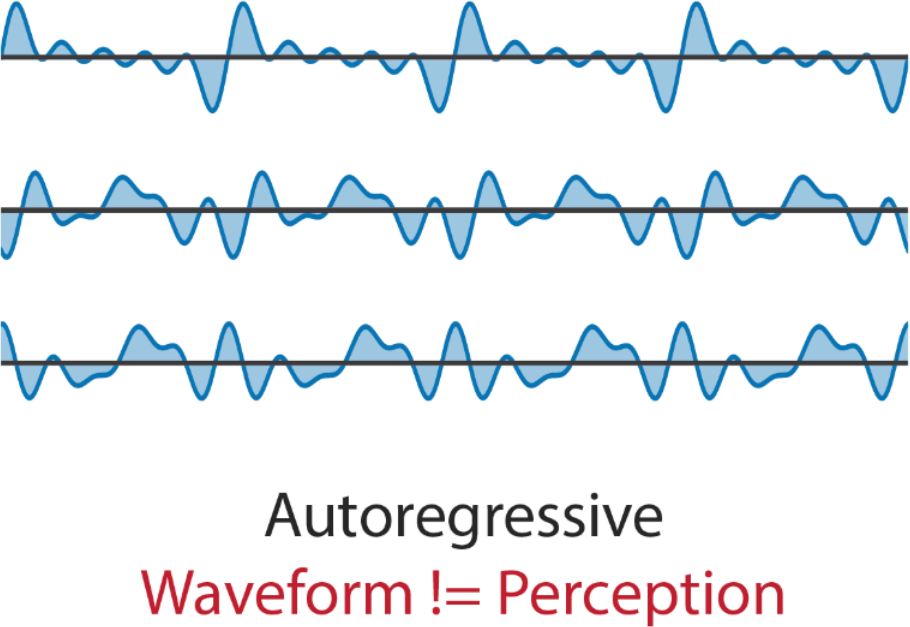
\includegraphics[width=0.5\linewidth]{rys03/d_dsp_example_graph.png}
    \caption{
      Przykład trzech próbek dźwięku, które dla słuchacza brzmią identycznie, mimo
      znacznych różnic w kształcie fali. Źródło obrazka: \cite{engel2020ddsp}.
    }
    \label{fig:waveform_not_equal_to_perception}
\end{figure}

\section{Porównanie barwy dźwięku w literaturze}

Żadna z prac przeanalizowanych podczas przeglądu literatury
(\cite{engel2020ddsp}, \cite{ieee_synth_programming}, \cite{ddx7}, \cite{riffusion},
\cite{evolutionary_puredata}, \cite{parallel_evolutionary_optimization_synth_parameters})
nie wykorzystuje metod porównywania sygnału osadzonych jedynie w dziedzinie czasu, ponieważ
nie są one skuteczne do porównywania dźwięków pod względem odczuć psychoakustycznych.
Przykład różnych kształtów fali, które z perspektywy słuchacza brzmią jak
taki sam dźwięk zademonstrowano na rysunku~\ref{fig:waveform_not_equal_to_perception}.

